%hablar un poco mas de utternaces.

Para la generación de utternaces, tanto de los audios en ingles como en castellano, utilizamos los repertorios fonéticos brindados por festvox (ver apéndice 1).

El primer desafío que se presenta es que estos repertorios fonéticos no tienen un mapeo directo con el Alfabeto Fonético Internacional: por ejemplo con este repertorio fonético, en el castellano existen tres fonos distintos para la /i/. Esta decisión por parte de festvox proviene de la necesidad de poder diferenciar la /i/ acentuada de la no acentuada  y de aquella presente en los diptongos: /ia/, /ie/, /io/, /iu/.

\begin{table}
\centering
%\setlength{\tabcolsep}{6pt} % default value is 6pt
\caption{Repertorios Foneticos utilizados por Festvox para Ingles y Castellano}
\begin{minipage}[t]{0.3\textwidth}
\begin{tabular}[t]{cc}
\toprule
Castellano & Ingles \\
\midrule
a & aa \\ 
a1 & ae \\ 
b & ah \\ 
ch & ao \\ 
d & aw \\ 
e & ax \\ 
e1 & ay \\ 
f & b \\ 
g & ch \\ 
i & d \\ 
i0 & s \\ 
i1 & dh \\ 
k & eh \\ 
l & er \\ 
ll & ey \\ 
m & f \\ 
n & g \\ 
ny & hh \\ 
o & ih \\ 
o1 & iy \\ 
\bottomrule
\end{tabular}
\end{minipage}
\begin{minipage}[t]{0.3\textwidth}
\begin{tabular}[t]{cc}
\toprule
Castellano & Ingles \\ 
\midrule
p & jh \\ 
r & k \\ 
rr & l \\ 
s & m \\  
t & n \\ 
u & ng \\ 
u0 & ow \\  
u1 & oy \\ 
 & p \\ 
 & r \\ 
 & sh \\ 
 &t \\ 
 &th \\ 
 &uh \\ 
 &uw \\ 
 &v \\ 
 &w \\ 
 &y \\ 
 &z \\ 
 &zh \\ 
\bottomrule
\end{tabular}
\end{minipage}
\end{table}

De aquí surgen varios problemas, el primero de los cuales es que festival utiliza el mismo simbolo para dos fonos distintos. De esta manera, la /g/ en castellano es suena mucho mas disminuida que la /g/ del repertorio ingles, aunque ambas sean descritas como un fono oclusivo velar sonoro.

De esto, surge el siguente problema: como sintetizar oraciones en castellano utilizando un repertorio fonético en ingles, donde incluso la cantidad de fonos es diferente. La manera que encontramos de abordar esto fue confeccionando de manera perceptual una tabla donde cada fonema del castellano estuviera mapeado a uno del ingles. En otras palabras, antes del entrenamiento del modelo, tomamos los fonos generados por festival para el corpus en ingles y los reemplazamos con fonos del castellano, a partir de la siguiente tabla:
\begin{table}
\centering
%\setlength{\tabcolsep}{6pt} % default value is 6pt
\caption{Mapeo Fonetico}
\begin{minipage}[t]{0.3\textwidth}
\begin{tabular}[t]{c|c}
\toprule
Ingles & Castellano \\
\midrule
ae & a\\  
aa & a1\\  
b & b\\  
ch & ch\\  
d & d\\  
dh & d\\  
eh & e\\  
el & e1\\  
f & f\\  
hh & g\\  
iy & i\\  
%FALTA i0
ih & i1\\  
k & k\\  
l & l\\  
jh & ll\\  
m & m\\  
n & n\\  
nx & n\\  
ao & o\\  
ou & o1\\  
p & p\\  
r & r/rr\\  
\bottomrule
\end{tabular}
\end{minipage}
\begin{minipage}[t]{0.3\textwidth}
\begin{tabular}[t]{c|c}
\toprule
Ingles & Castellano \\ 
\midrule
s & s\\  
t & t\\  
uw & u\\  
w & u0\\  
uh & u1\\  
dx & -\\  
em & -\\  
en & -\\  
er & -\\  
ei & -\\  
g & -\\  
hv & -\\  
ng & -\\  
th & -\\  
v & -\\  
y & -\\  
sh & -\\  
zh & -\\  
z  & -\\  
\bottomrule
\end{tabular}
\end{minipage}
\end{table}

Por otro lado para varios fonos tuvimos que hacer reglas especiales ya que no contabamos con ningun fono del ingles lo suficientemente similar. Así,  para el fono ny (ñ o \textltailn en ipa) colapsamos las apariciones del fono /n/ seguido de /j/. Si bien esta solución puede parecer algo forzada, ya que estamos generando de manera casera fonos a partir de otros, consideramos que esto se aproxima en cierta medida a la manera real en la que un hablante no nativo aprende un idioma con una carga fonética diferente al suyo. Citando un extracto del trabajo \textit{Transcription of Spanish and Spanish-Influenced English, Brian Goldstein, Temple University}:

\begin{center}
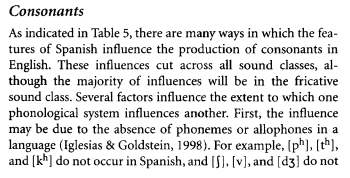
\includegraphics[scale=0.5]{imagenes_investigacion/consonantes1.png}
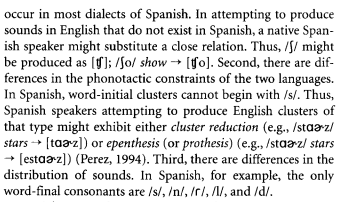
\includegraphics[scale=0.5]{imagenes_investigacion/consonantes2.png}
\end{center}

Visto desde nuestra perspectiva, una persona que aprende una nueva lengua, realiza una aproximación entre los fonos conocidos y los fonos `objetivo' de la nueva lengua.

De manera similar el ingles carece del fono vibrante múltiple alveolar sordo /\textipa{r}/ y dado que el fono /\textipa{R}/ ya estaba siendo utilizado, no podíamos realizar un mapeo tan directo. Como sulución tomamos la mitad de los fonos /\textipa{R}/ y los remplazamos con /\textipa{r}/. Un problema similar surge del fono /g/, que si bien este existe en ingles, al utilizarlo para sintetizar oraciones sonaba muy alienigena. Con el objetivo de suavizar el sonido tomamos el fono de la /g/ y lo mapeamos a un fono que no fuera utilizado y tomamos los fonos etiquetados con /hh/ del ingles y los remplazamos con el /g/ del castellano.

Aquellos fonos que consideramos suficientemente disimiles del castellano, como es el caso de la /sh/, /z/, etc los mapeamos a caracteres que no interfirieran para el entrenamiento ya que no los utilizaremos para la sintesis.

Utilizando estos fonos a la hora de entrenar nos permite sintetizar oraciones en castellano, aunque como es de esperar, dado que el corpus de entrenamiento es tan disimilar de las oraciones que queremos sintetizar, donde tanto las combinaciones de fonemas, las reglas prosodicas y las acentuaciónes vocalicas son distintas, los audios sitetizados resultan incomprensibles y de muy baja calidad

% mapeo utilizado mostrar.
% el etiquetado de cmu\_arctic es en ingles y mapeando al castellano.